% Results
\section{Results}
\label{sec:results}

\subsection{In-Domain Accuracy on KITTI}
\label{sec:results_kitti}

Table~\ref{tab:kitti_results} reports the KITTI in-domain results for the four detectors.
YOLOv8s achieves the highest accuracy on every axis, with mAP@$[0.50{:}0.95]$ of $0.690$,
AP50 of $0.925$, and AP75 of $0.780$. The accuracy ranking is YOLOv8s
($0.690$) $>$ RT-DETR-L ($0.606$) $>$ Faster R-CNN ($0.589$) $>$ RetinaNet ($0.537$).
Pedestrian is the weakest class across all four detectors ($0.392$--$0.530$), consistent
with the class's small object size and limited training instances, while Vehicle is the
strongest ($0.703$--$0.849$).

\begin{figure}[t]
    \centering
    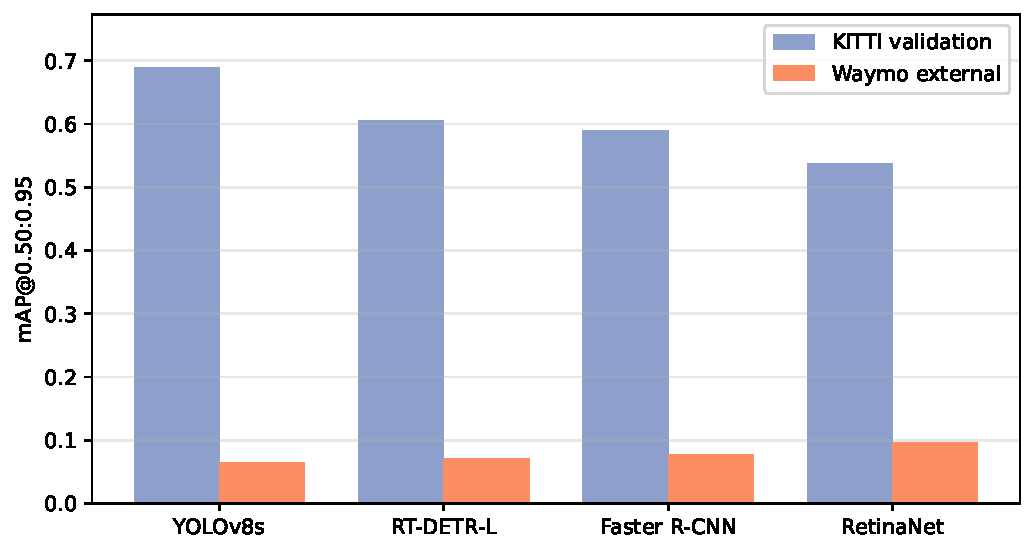
\includegraphics[width=\linewidth]{figures/kitti_vs_waymo_map50_95.pdf}
    \caption{KITTI in-domain versus Waymo external mAP@$[0.50{:}0.95]$ under target-free
    transfer. All detectors degrade sharply, and the in-domain ranking does not transfer to
    the external setting.}
    \label{fig:kitti_vs_waymo}
\end{figure}

\begin{table}[t]
    \centering
    \caption{KITTI in-domain detection results on the frozen validation split (1{,}496 images). Values are COCO Average Precision.}
    \label{tab:kitti_results}
    \begin{tabular}{lcccccc}
        \toprule
        Detector & mAP@0.50:0.95 & mAP@0.50 & mAP@0.75 & Vehicle AP & Pedestrian AP & Cyclist AP \\
        \midrule
        YOLOv8s & 0.690 & 0.925 & 0.780 & 0.849 & 0.530 & 0.691 \\
        RT-DETR-L & 0.606 & 0.906 & 0.679 & 0.730 & 0.490 & 0.597 \\
        Faster R-CNN & 0.589 & 0.879 & 0.666 & 0.741 & 0.432 & 0.594 \\
        RetinaNet & 0.537 & 0.839 & 0.577 & 0.703 & 0.392 & 0.518 \\
        \bottomrule
    \end{tabular}
\end{table}


\subsection{Computational Efficiency}
\label{sec:results_efficiency}

Table~\ref{tab:efficiency} summarizes the deployment-oriented efficiency comparison on the
local GPU. YOLOv8s is by far the most efficient detector: $11.1$M parameters, a $21.5$~MB
checkpoint, $12.36$~ms latency, and $94.77$~FPS. RT-DETR-L offers the second-best accuracy
but is considerably slower ($55.29$~ms, $18.73$~FPS). The two heaviest detectors carry a
large efficiency penalty: Faster R-CNN ($41.3$M parameters, $315.68$~MB, $91.22$~ms) and
RetinaNet ($36.4$M parameters, $278.0$~MB, $75.25$~ms).

\begin{table}[t]
    \centering
    \caption{Deployment-oriented efficiency comparison on the local GPU.}
    \label{tab:efficiency}
    \begin{tabular}{lcccc}
        \toprule
        Detector & Parameters (M) & Checkpoint (MB) & Latency (ms) & FPS \\
        \midrule
        YOLOv8s & 11.1 & 21.50 & 12.36 & 94.77 \\
        RT-DETR-L & 32.8 & 63.15 & 55.29 & 18.73 \\
        Faster R-CNN & 41.3 & 315.68 & 91.22 & 11.24 \\
        RetinaNet & 36.4 & 278.00 & 75.25 & 13.70 \\
        \bottomrule
    \end{tabular}
\end{table}


\subsection{Operating-Point Behavior}
\label{sec:results_operating_point}

At the fixed operating point (confidence $\geq 0.25$, IoU $\geq 0.50$,
Table~\ref{tab:operating_point}), YOLOv8s attains the highest precision ($0.926$) with a
high recall ($0.947$). RT-DETR-L emits many low-confidence detections (DETR-style
$300$ queries), so it achieves the highest recall ($0.969$) but the lowest precision
($0.482$) and the most false positives per image ($5.431$). Faster R-CNN and RetinaNet
fall between these two extremes.

\begin{table}[t]
    \centering
    \caption{Operating-point metrics on KITTI validation (confidence $\geq 0.25$, IoU $\geq 0.50$).}
    \label{tab:operating_point}
    \begin{tabular}{lcccc}
        \toprule
        Detector & Precision & Recall & F1 & FP/image \\
        \midrule
        YOLOv8s & 0.926 & 0.947 & 0.936 & 0.40 \\
        RT-DETR-L & 0.482 & 0.969 & 0.643 & 5.43 \\
        Faster R-CNN & 0.876 & 0.928 & 0.901 & 0.69 \\
        RetinaNet & 0.777 & 0.907 & 0.837 & 1.35 \\
        \bottomrule
    \end{tabular}
\end{table}


\subsection{Cross-Dataset External Validation on Waymo}
\label{sec:results_waymo}

Table~\ref{tab:waymo_results} reports the Waymo external-validation results obtained by
applying the four KITTI-trained checkpoints directly to the frozen Waymo subset with no
retraining. All detectors degrade sharply: mAP@$[0.50{:}0.95]$ falls to
$0.065$--$0.097$, an order of magnitude below the KITTI baseline
(Figure~\ref{fig:kitti_vs_waymo}). RetinaNet achieves the highest Waymo accuracy
($0.097$), followed by Faster R-CNN ($0.077$), RT-DETR-L ($0.071$), and YOLOv8s ($0.065$),
the reverse of the in-domain ranking.

\begin{table}[t]
    \centering
    \caption{Waymo external-validation results (996 front-camera images, no retraining).}
    \label{tab:waymo_results}
    \begin{tabular}{lcccccc}
        \toprule
        Detector & mAP@0.50 & mAP@0.50:0.95 & Vehicle AP & Pedestrian AP & Cyclist AP & Mean inf. (ms) \\
        \midrule
        YOLOv8s & 0.142 & 0.065 & 0.106 & 0.049 & 0.042 & 34.21 \\
        RT-DETR-L & 0.151 & 0.071 & 0.116 & 0.058 & 0.041 & 62.57 \\
        Faster R-CNN & 0.175 & 0.077 & 0.123 & 0.070 & 0.038 & 92.07 \\
        RetinaNet & 0.215 & 0.097 & 0.144 & 0.075 & 0.072 & 77.50 \\
        \bottomrule
    \end{tabular}
\end{table}


Table~\ref{tab:kitti_vs_waymo} quantifies the degradation and the generalization ratio
(Waymo mAP divided by KITTI mAP). Relative mAP@$[0.50{:}0.95]$ drops range from $82.0\%$
(RetinaNet) to $90.5\%$ (YOLOv8s), and generalization ratios range from $0.095$ (YOLOv8s)
to $0.180$ (RetinaNet), as shown in Figure~\ref{fig:generalization_ratio}. The best
generalizing detector is RetinaNet and the worst is YOLOv8s.

\begin{figure}[t]
    \centering
    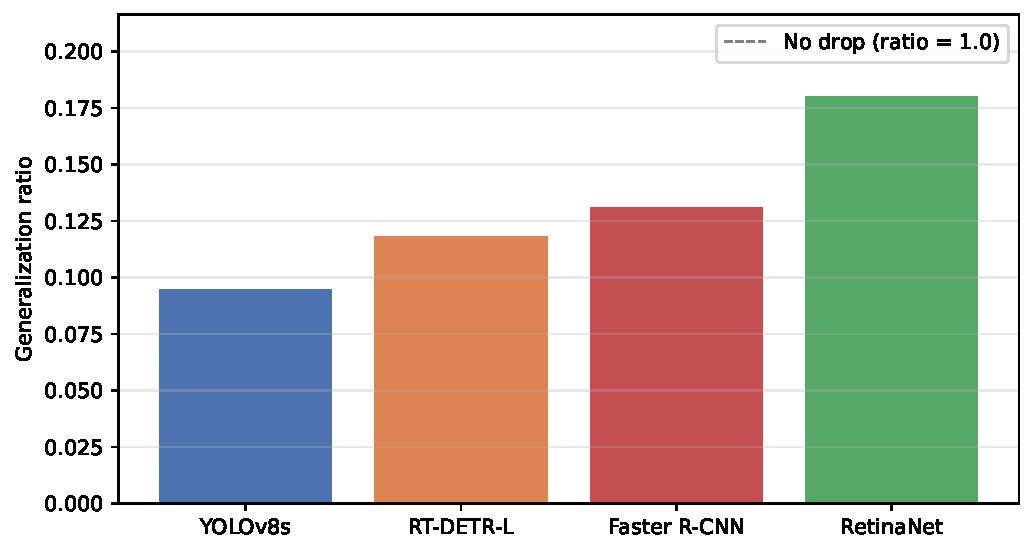
\includegraphics[width=\linewidth]{figures/generalization_ratio_map50_95.pdf}
    \caption{Generalization ratio (Waymo mAP@$[0.50{:}0.95]$ / KITTI mAP@$[0.50{:}0.95]$)
    for the four detectors. Higher values indicate greater cross-domain stability.}
    \label{fig:generalization_ratio}
\end{figure}

\begin{table}[t]
    \centering
    \caption{KITTI-to-Waymo degradation in mAP@0.50:0.95 and generalization ratio.}
    \label{tab:kitti_vs_waymo}
    \begin{tabular}{lccccc}
        \toprule
        Detector & KITTI mAP & Waymo mAP & Abs. drop & Drop (\%) & Gen. ratio \\
        \midrule
        YOLOv8s & 0.690 & 0.065 & 0.625 & 90.52 & 0.095 \\
        RT-DETR-L & 0.606 & 0.071 & 0.534 & 88.21 & 0.118 \\
        Faster R-CNN & 0.589 & 0.077 & 0.512 & 86.92 & 0.131 \\
        RetinaNet & 0.538 & 0.097 & 0.441 & 81.98 & 0.180 \\
        \bottomrule
    \end{tabular}
\end{table}


\subsection{Class-Wise Degradation}
\label{sec:results_class_wise}

Table~\ref{tab:class_wise_degradation} reports per-class AP@$[0.50{:}0.95]$ on both
datasets together with the absolute and relative drop. Vehicle exhibits the largest
absolute drop across detectors (Figure~\ref{fig:class_wise_degradation}), reflecting its
high in-domain score combined with a large distributional shift in scale and appearance on
Waymo. Cyclist shows the largest relative drop (up to $94.0\%$), while Pedestrian degrades
least in absolute terms but from a low baseline.

\begin{figure}[t]
    \centering
    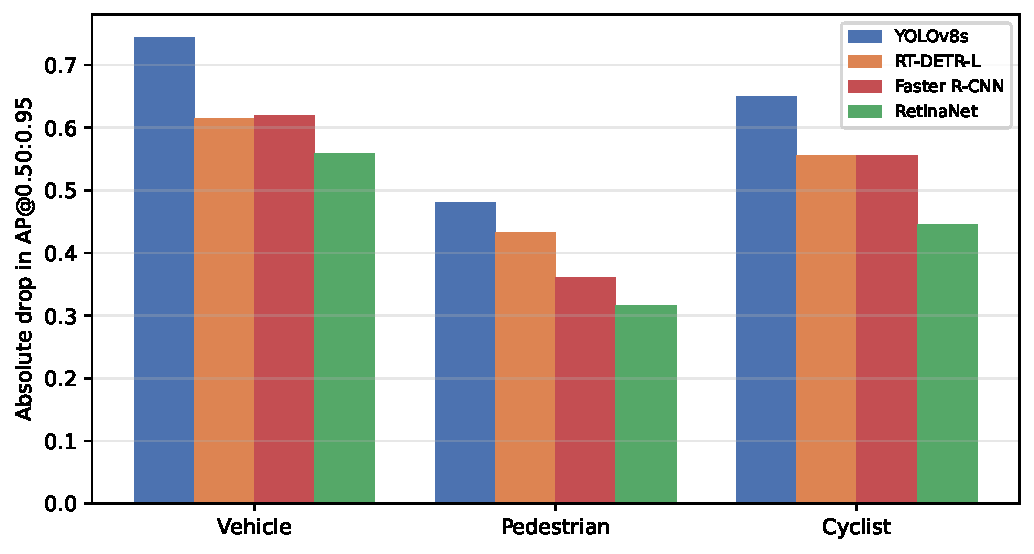
\includegraphics[width=\linewidth]{figures/class_wise_degradation.pdf}
    \caption{Class-wise absolute degradation in AP@$[0.50{:}0.95]$ (KITTI minus Waymo) by
    detector.}
    \label{fig:class_wise_degradation}
\end{figure}

\begin{table}[t]
    \centering
    \caption{Class-wise cross-dataset degradation in AP@0.50:0.95.}
    \label{tab:class_wise_degradation}
    \begin{tabular}{llcccc}
        \toprule
        Detector & Class & KITTI AP & Waymo AP & Abs. drop & Drop (\%) \\
        \midrule
        YOLOv8s & Vehicle & 0.849 & 0.106 & 0.743 & 87.56 \\
         & Pedestrian & 0.530 & 0.049 & 0.481 & 90.74 \\
         & Cyclist & 0.691 & 0.042 & 0.649 & 93.98 \\
        \addlinespace
        RT-DETR-L & Vehicle & 0.730 & 0.116 & 0.615 & 84.17 \\
         & Pedestrian & 0.490 & 0.058 & 0.432 & 88.20 \\
         & Cyclist & 0.597 & 0.041 & 0.556 & 93.15 \\
        \addlinespace
        Faster R-CNN & Vehicle & 0.741 & 0.123 & 0.619 & 83.46 \\
         & Pedestrian & 0.432 & 0.070 & 0.362 & 83.74 \\
         & Cyclist & 0.594 & 0.038 & 0.556 & 93.54 \\
        \addlinespace
        RetinaNet & Vehicle & 0.703 & 0.144 & 0.559 & 79.54 \\
         & Pedestrian & 0.391 & 0.075 & 0.317 & 80.93 \\
         & Cyclist & 0.518 & 0.072 & 0.446 & 86.08 \\
        \bottomrule
    \end{tabular}
\end{table}


\subsection{Robustness and Safety-Oriented Analysis}
\label{sec:results_safety}

\subsubsection{Object-Size Analysis}
\label{sec:results_size}

Recall and miss rate were computed per detector, dataset, and size category at the
operating point (Table~\ref{tab:object_size_recall}). On KITTI, recall declines with
object size but remains high for all detectors ($0.88$--$0.96$ small-object recall); on
Waymo, small-object recall collapses, reaching $0.045$--$0.132$ across detectors
(Figure~\ref{fig:object_size_recall}). This indicates that small objects are the dominant
failure mode under domain shift, consistent with Waymo containing many more small and
distant objects.

\begin{figure}[t]
    \centering
    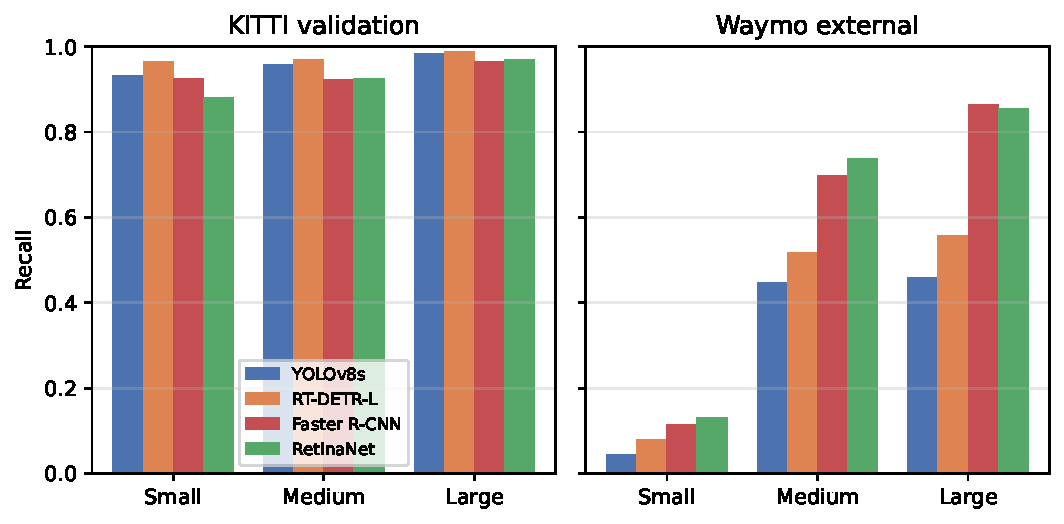
\includegraphics[width=\linewidth]{figures/object_size_recall.pdf}
    \caption{Recall by object-size category at the operating point for KITTI (left) and
    Waymo (right).}
    \label{fig:object_size_recall}
\end{figure}

\begin{table}[t]
    \centering
    \caption{Class-agnostic recall by object-size category at the frozen operating point (confidence $\geq 0.25$, IoU $\geq 0.50$).}
    \label{tab:object_size_recall}
    \begin{tabular}{lcccccc}
        \toprule
        Detector & \multicolumn{3}{c}{KITTI recall} & \multicolumn{3}{c}{Waymo recall} \\
        & Small & Medium & Large & Small & Medium & Large \\
        \midrule
        YOLOv8s & 0.932 & 0.958 & 0.985 & 0.045 & 0.448 & 0.460 \\
        RT-DETR-L & 0.964 & 0.971 & 0.989 & 0.081 & 0.517 & 0.558 \\
        Faster R-CNN & 0.925 & 0.923 & 0.966 & 0.115 & 0.697 & 0.865 \\
        RetinaNet & 0.881 & 0.926 & 0.970 & 0.132 & 0.737 & 0.855 \\
        \bottomrule
    \end{tabular}
\end{table}


\subsubsection{Safety-Critical False Negatives}
\label{sec:results_safety_fn}

False-negative rates for the safety-priority classes (Pedestrian and Cyclist) were computed
separately from overall accuracy (Table~\ref{tab:safety_fn}). On Waymo, the combined
pedestrian-plus-cyclist false-negative rate is $0.81$--$0.93$ for all detectors
(Figure~\ref{fig:pedestrian_cyclist_fn}), a safety-relevant result that is not visible
from average mAP alone: even the detector with the best Waymo mAP misses the large majority
of vulnerable road users.

\begin{figure}[t]
    \centering
    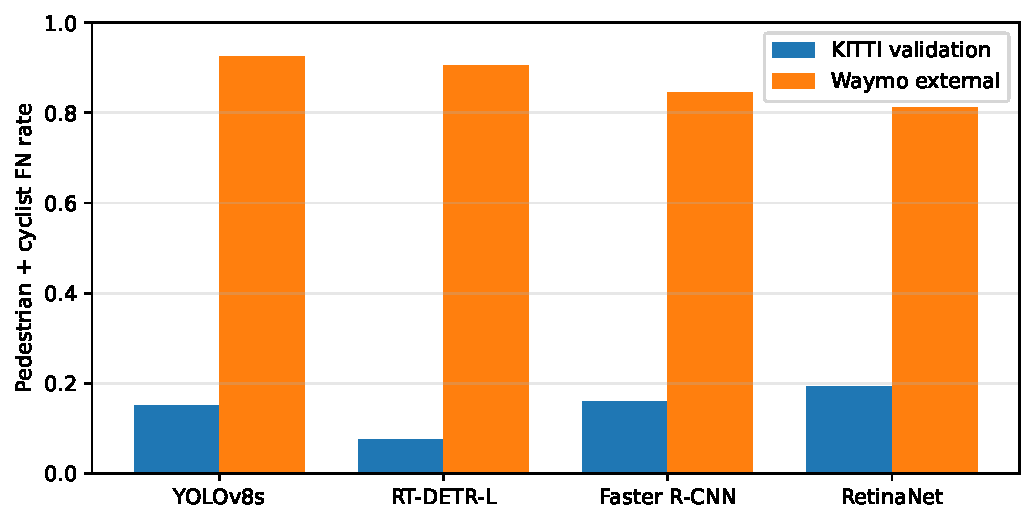
\includegraphics[width=\linewidth]{figures/pedestrian_cyclist_fn_rate.pdf}
    \caption{Safety-critical false-negative rate for pedestrians and cyclists at the
    operating point, for KITTI and Waymo.}
    \label{fig:pedestrian_cyclist_fn}
\end{figure}

\begin{table}[t]
    \centering
    \caption{Safety-critical false-negative rate for pedestrians and cyclists (operating point, confidence $\geq 0.25$, IoU $\geq 0.50$).}
    \label{tab:safety_fn}
    \begin{tabular}{lcc}
        \toprule
        Detector & KITTI FN rate & Waymo FN rate \\
        \midrule
        YOLOv8s & 0.152 & 0.926 \\
        RT-DETR-L & 0.077 & 0.906 \\
        Faster R-CNN & 0.159 & 0.844 \\
        RetinaNet & 0.194 & 0.811 \\
        \bottomrule
    \end{tabular}
\end{table}


\subsubsection{Failure-Type Decomposition}
\label{sec:results_failure_type}

Table~\ref{tab:failure_type} decomposes detections into true positives, missed detections,
false positives, localization errors, class confusions, and over-detections. On KITTI,
RT-DETR-L emits the most false positives and by far the most over-detections, consistent
with its low operating-point precision. On Waymo, missed detections dominate for every
detector, again reflecting the collapse of small-object recall.

\begin{table}[t]
    \centering
    \caption{Failure-type decomposition at the operating point for KITTI and Waymo.}
    \label{tab:failure_type}
    \begin{tabular}{llcccccc}
        \toprule
        Dataset & Detector & TP & Miss (FN) & FP & Localization & Confusion & Over-detect. \\
        \midrule
        KITTI & YOLOv8s & 7,382 & 410 & 163 & 272 & 15 & 142 \\
         & RT-DETR-L & 7,551 & 241 & 777 & 1,620 & 82 & 5,646 \\
         & Faster R-CNN & 7,231 & 561 & 241 & 592 & 96 & 98 \\
         & RetinaNet & 7,069 & 723 & 425 & 1,165 & 161 & 274 \\
        \addlinespace
        Waymo & YOLOv8s & 2,721 & 22,098 & 20 & 132 & 56 & 27 \\
         & RT-DETR-L & 3,769 & 21,050 & 40 & 446 & 132 & 743 \\
         & Faster R-CNN & 5,269 & 19,550 & 292 & 1,263 & 366 & 78 \\
         & RetinaNet & 5,771 & 19,048 & 328 & 2,007 & 561 & 216 \\
        \bottomrule
    \end{tabular}
\end{table}


\subsection{Deployment Trade-Off}
\label{sec:results_deployment}

Table~\ref{tab:deployment} and Figure~\ref{fig:deployment_tradeoff} jointly summarize
in-domain accuracy, external accuracy, latency, and vulnerable-road-user (VRU) safety on
Waymo (the VRU false-negative rate and the small-object recall restricted to pedestrians
and cyclists). No single detector simultaneously optimizes accuracy, generalization,
latency, and safety: YOLOv8s is fastest and most accurate in-domain but least stable and
safety-reliable out-of-domain, while RetinaNet generalizes best and is most safety-reliable
on Waymo but is slower and weaker in-domain.

\begin{figure}[t]
    \centering
    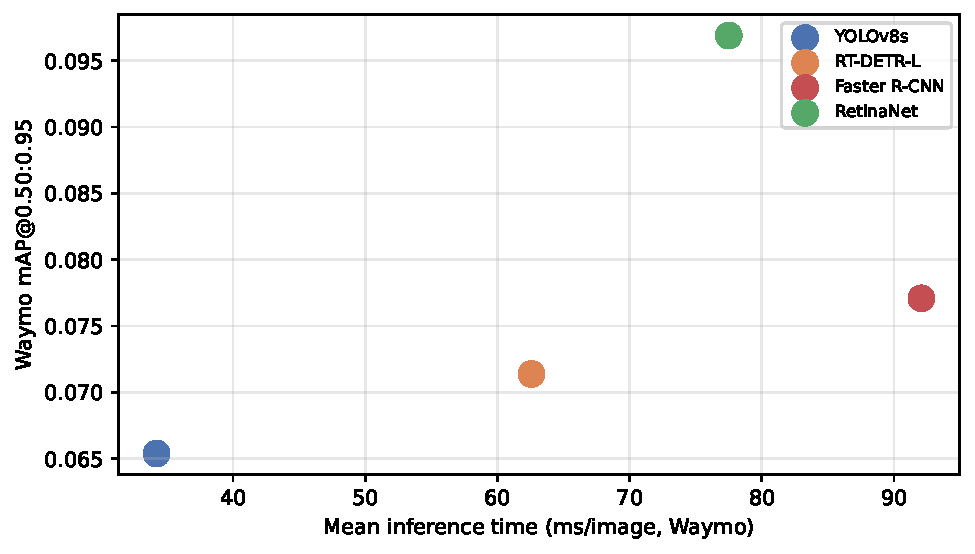
\includegraphics[width=\linewidth]{figures/deployment_tradeoff.pdf}
    \caption{Deployment trade-off between mean inference time and Waymo mAP@$[0.50{:}0.95]$.}
    \label{fig:deployment_tradeoff}
\end{figure}

\begin{table}[t]
    \centering
    \caption{Deployment trade-off: in-domain accuracy, external accuracy, latency, and vulnerable-road-user (VRU) safety on Waymo.}
    \label{tab:deployment}
    \begin{tabular}{lccccc}
        \toprule
        Detector & KITTI mAP & Waymo mAP & Latency (ms) & Waymo VRU FN & Waymo VRU small recall \\
        \midrule
        YOLOv8s & 0.690 & 0.065 & 34.21 & 0.926 & 0.029 \\
        RT-DETR-L & 0.606 & 0.071 & 62.57 & 0.906 & 0.047 \\
        Faster R-CNN & 0.589 & 0.077 & 92.07 & 0.844 & 0.097 \\
        RetinaNet & 0.537 & 0.097 & 77.50 & 0.811 & 0.127 \\
        \bottomrule
    \end{tabular}
\end{table}

